% answers.tex —— 2006 年·全国卷Ⅱ·理科 · 参考答案与详细解析片段
% 由 tools/generate_projects.py 依来源总账自 2006/2006_数学真题_全国2理_试题.md + 2006/2006_数学真题_全国2理_解析正文.md + 2006/2006_数学真题_全国2理_答案要点.md 生成，勿手改（改源 MD 后重跑）


\begin{gktip}
固定源 PDF 为印刷页码 316–317 的两页题面，不附答案。以下解析均依据固定源独立复算；第 7、16、19、21 题图形在 LaTeX 工程中以 TikZ/PGFPlots 矢量源重绘。
\end{gktip}

\begin{answer}
\gksolhead{1}{}

\textbf{题目}：

设集合 $M=\{x\mid x<3\}$，$N=\{x\mid\log_2x>1\}$，则 $M\cap N=$\mbox{（　　）}

（A）$\varnothing$\quad（B）$\{x\mid0<x<3\}$\quad（C）$\{x\mid1<x<3\}$\quad（D）$\{x\mid2<x<3\}$

\Needspace{4\baselineskip}
\textbf{解析}

由 $\log_2x>1$ 得 $x>2$，所以 $M\cap N=(2,3)$。

\gkanswer{答案：B}

\end{answer}
\begin{answer}
\gksolhead{2}{}

\textbf{题目}：

函数 $y=\sin2x\cos2x$ 的最小正周期是\mbox{（　　）}

（A）$2\pi$\quad（B）$4\pi$\quad（C）$\dfrac\pi4$\quad（D）$\dfrac\pi2$

\Needspace{4\baselineskip}
\textbf{解析}

\nopagebreak[4]
\[
\sin2x\cos2x=\frac12\sin4x\text{，}
\]

故最小正周期为 $\dfrac\pi2$。

\gkanswer{答案：C}

\end{answer}
\begin{answer}
\gksolhead{3}{}

\textbf{题目}：

$\dfrac{3}{(1-i)^2}=$\mbox{（　　）}

（A）$\dfrac32i$\quad（B）$-\dfrac32i$\quad（C）$i$\quad（D）$-i$

\Needspace{4\baselineskip}
\textbf{解析}

\nopagebreak[4]
\[
(1-i)^2=-2i\text{，}\qquad \frac3{(1-i)^2}=\frac3{-2i}=\frac32i\text{。}
\]

\gkanswer{答案：A}

\end{answer}
\begin{answer}
\gksolhead{4}{}

\textbf{题目}：

过球的一条半径的中点，作垂直于该半径的平面，则所得截面的面积与球的表面积的比为\mbox{（　　）}

（A）$\dfrac3{16}$\quad（B）$\dfrac9{16}$\quad（C）$\dfrac38$\quad（D）$\dfrac9{32}$

\Needspace{4\baselineskip}
\textbf{解析}

\Needspace{5\baselineskip}
设球半径为 $R$，截面圆心到球心的距离为 $R/2$。截面半径为 $\dfrac{\sqrt3}{2}R$，所以面积比为

\nopagebreak[4]
\[
\frac{\pi(\sqrt3R/2)^2}{4\pi R^2}=\frac3{16}\text{。}
\]

\gkanswer{答案：A}

\end{answer}
\begin{answer}
\gksolhead{5}{}

\textbf{题目}：

已知 $\triangle ABC$ 的顶点 $B,C$ 在椭圆 $\dfrac{x^2}{3}+y^2=1$ 上，顶点 $A$ 是椭圆的一个焦点，且椭圆的另外一个焦点在 $BC$ 边上，则 $\triangle ABC$ 的周长是\mbox{（　　）}

（A）$2\sqrt3$\quad（B）$6$\quad（C）$4\sqrt3$\quad（D）$12$

\Needspace{4\baselineskip}
\textbf{解析}

与全国卷Ⅱ文科第 5 题相同，利用椭圆定义得到三角形周长为 $4\sqrt3$。

\gkanswer{答案：C}

\end{answer}
\begin{answer}
\gksolhead{6}{}

\textbf{题目}：

已知函数 $f(x)=\ln x+1\ (x>0)$，则 $f(x)$ 的反函数为\mbox{（　　）}

（A）$y=e^{x+1}\ (x\in\mathbb R)$\quad（B）$y=e^{x-1}\ (x\in\mathbb R)$

（C）$y=e^{x+1}\ (x>1)$\quad（D）$y=e^{x-1}\ (x>1)$

\Needspace{4\baselineskip}
\textbf{解析}

由 $y=\ln x+1$ 反解得 $x=e^{y-1}$，交换变量后反函数为 $y=e^{x-1}\ (x>1)$。

\gkanswer{答案：D}

\end{answer}
\begin{answer}
\gksolhead{7}{}

\textbf{题目}：

如图，平面 $\alpha\perp$ 平面 $\beta$，$A\in\alpha$，$B\in\beta$，$AB$ 与两平面 $\alpha,\beta$ 所成的角分别为 $\dfrac\pi4$ 和 $\dfrac\pi6$。过 $A,B$ 分别作两平面交线的垂线，垂足为 $A',B'$，则 $AB:A'B'=$\mbox{（　　）}
\nopagebreak[4]
\begin{center}% 2006 年全国卷Ⅱ理科第 7 题：两个互相垂直的平面
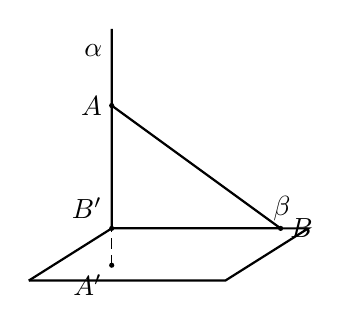
\begin{tikzpicture}[>=stealth,scale=0.78]
  \coordinate (I) at (0,0);
  \coordinate (J) at (1.35,0.85);
  \coordinate (K) at (4.55,0.85);
  \coordinate (L) at (3.20,0);
  \coordinate (Atop) at (1.35,4.10);
  \coordinate (A) at (1.35,2.85);
  \coordinate (Aprime) at (1.35,0.25);
  \coordinate (Bprime) at (1.35,0.85);
  \coordinate (B) at (4.10,0.85);
  \draw[thick] (I)--(J)--(Atop);
  \draw[thick] (I)--(L)--(K)--(J);
  \draw[thick] (J)--(B);
  \draw[thick] (A)--(B);
  \draw[dashed] (A)--(Aprime) (Aprime)--(Bprime);
  \fill (A) circle (1.2pt) node[left] {$A$};
  \fill (Aprime) circle (1.2pt) node[below left] {$A'$};
  \fill (Bprime) circle (1.2pt) node[above left] {$B'$};
  \fill (B) circle (1.2pt) node[right] {$B$};
  \node at (1.05,3.75) {$\alpha$};
  \node at (4.12,1.18) {$\beta$};
\end{tikzpicture}
\end{center}
\nopagebreak[4]
（A）$2:1$\quad（B）$3:1$\quad（C）$3:2$\quad（D）$4:3$

\Needspace{4\baselineskip}
\textbf{解析}

\Needspace{5\baselineskip}
设 $AB=L$。其垂直于两个互相垂直平面的分量分别为 $L\sin\dfrac\pi4$、$L\sin\dfrac\pi6$，沿两平面交线方向的分量就是 $A'B'$，故

\nopagebreak[4]
\[
A'B'=\sqrt{L^2-\frac{L^2}{2}-\frac{L^2}{4}}=\frac L2\text{，}
\]

从而 $AB:A'B'=2:1$。

\gkanswer{答案：A}

\end{answer}
\begin{answer}
\gksolhead{8}{}

\textbf{题目}：

已知函数 $y=f(x)$ 的图象与函数 $g(x)=\log_2x\ (x>0)$ 的图象关于原点对称，则 $f(x)$ 的表达式为\mbox{（　　）}

（A）$f(x)=\dfrac1{\log_2x}\ (x>0)$\quad（B）$f(x)=\dfrac1{\log_2(-x)}\ (x<0)$

（C）$f(x)=-\log_2x\ (x>0)$\quad（D）$f(x)=-\log_2(-x)\ (x<0)$

\Needspace{4\baselineskip}
\textbf{解析}

\Needspace{5\baselineskip}
设 $g(x)=\log_2x$。图象关于原点对称后，点 $(u,g(u))$ 变为 $(-u,-g(u))$。因此在 $x<0$ 时

\nopagebreak[4]
\[
f(x)=-\log_2(-x)\text{。}
\]

\gkanswer{答案：D}

\end{answer}
\begin{answer}
\gksolhead{9}{}

\textbf{题目}：

已知双曲线 $\dfrac{x^2}{a^2}-\dfrac{y^2}{b^2}=1$ 的一条渐近线方程为 $y=\dfrac43x$，则双曲线的离心率为\mbox{（　　）}

（A）$\dfrac53$\quad（B）$\dfrac43$\quad（C）$\dfrac54$\quad（D）$\dfrac32$

\Needspace{4\baselineskip}
\textbf{解析}

\Needspace{5\baselineskip}
渐近线斜率给出 $b/a=4/3$，故

\nopagebreak[4]
\[
e=\sqrt{1+\frac{b^2}{a^2}}=\frac53\text{。}
\]

\gkanswer{答案：A}

\end{answer}
\begin{answer}
\gksolhead{10}{}

\textbf{题目}：

若 $f(\sin x)=3-\cos2x$，则 $f(\cos x)=$\mbox{（　　）}

（A）$3-\cos2x$\quad（B）$3-\sin2x$\quad（C）$3+\cos2x$\quad（D）$3+\sin2x$

\Needspace{4\baselineskip}
\textbf{解析}

由 $f(\sin x)=2+2\sin^2x$ 得 $f(u)=2+2u^2$，所以 $f(\cos x)=3+\cos2x$。

\gkanswer{答案：C}

\end{answer}
\begin{answer}
\gksolhead{11}{}

\textbf{题目}：

设 $S_n$ 是等差数列 $\{a_n\}$ 的前 $n$ 项和，若 $\dfrac{S_3}{S_6}=\dfrac13$，则 $\dfrac{S_6}{S_{12}}=$\mbox{（　　）}

（A）$\dfrac3{10}$\quad（B）$\dfrac13$\quad（C）$\dfrac18$\quad（D）$\dfrac19$

\Needspace{4\baselineskip}
\textbf{解析}

设切点横坐标为 $t$，切线为 $y=(2t+1)x+1-t^2$。令其经过 $(-1,0)$，得到 $t(t+2)=0$。取 $t=0$ 时切线为 $x-y+1=0$。

\gkanswer{答案：A}

\end{answer}
\begin{answer}
\gksolhead{12}{}

\textbf{题目}：

函数 $\displaystyle\sum_{n=1}^{19}|x-n|$ 的最小值为\mbox{（　　）}

（A）$190$\quad（B）$171$\quad（C）$90$\quad（D）$45$

\Needspace{4\baselineskip}
\textbf{解析}

\Needspace{5\baselineskip}
函数 $\sum_{n=1}^{19}|x-n|$ 在数据的中位数 $x=10$ 处取最小值，最小值为

\nopagebreak[4]
\[
2(1+2+\cdots+9)=90\text{。}
\]

\gkanswer{答案：C}

\end{answer}
\begin{answer}
\gksolhead{13}{}

\textbf{题目}：

在 $\left(x^4+\dfrac1x\right)^{10}$ 的展开式中常数项是\gkblank{}。（用数字作答）

\Needspace{4\baselineskip}
\textbf{解析}

常数项要求 $4(10-k)-k=0$，所以 $k=8$，常数项为 $\binom{10}{8}=45$。

\gkanswer{答案：$45$}

\end{answer}
\begin{answer}
\gksolhead{14}{}

\textbf{题目}：

已知 $\triangle ABC$ 的三个内角 $A,B,C$ 成等差数列，且 $AB=1,BC=4$，则边 $BC$ 上的中线 $AD$ 的长为\gkblank{}。

\Needspace{4\baselineskip}
\textbf{解析}

\Needspace{5\baselineskip}
三个角成等差数列且和为 $\pi$，所以 $B=\dfrac\pi3$。由正弦定理及已知 $AB=1,BC=4$，可得 $CA=\sqrt{13}$。于是以 $BC$ 为底边的中线满足

\nopagebreak[4]
\[
AD=\frac12\sqrt{2AB^2+2AC^2-BC^2}=\frac12\sqrt{2+26-16}=\sqrt3\text{。}
\]

\gkanswer{答案：$\sqrt3$}

\end{answer}
\begin{answer}
\gksolhead{15}{}

\textbf{题目}：

过点 $(1,\sqrt2)$ 的直线 $l$ 将圆 $(x-2)^2+y^2=4$ 分成两段弧，当劣弧所对的圆心角最小时，直线 $l$ 的斜率 $k=$\gkblank{}。

\Needspace{4\baselineskip}
\textbf{解析}

圆心为 $O(2,0)$，点 $P=(1,\sqrt2)$ 在圆内。过 $P$ 的弦长最小时，直线到圆心的距离最大，故直线垂直于 $OP$。$OP$ 斜率为 $-\sqrt2$，所求斜率为 $\dfrac{\sqrt2}{2}$。

\gkanswer{答案：$\dfrac{\sqrt2}{2}$}

\end{answer}
\begin{answer}
\gksolhead{16}{}

\textbf{题目}：

一个社会调查机构就某地居民的月收入调查了 $10000$ 人，并根据所得数据画了样本的频率分布直方图（如图）。为了分析居民的收入与年龄、学历、职业等方面的关系，要从这 $10000$ 人中再用分层抽样方法抽出 $100$ 人作进一步调查，则在 $[2500,3000)$（元）月收入段应抽出\gkblank{}人。
\nopagebreak[4]
\begin{center}% 2006 年全国卷Ⅱ理科第 16 题：月收入频率分布直方图
\begin{tikzpicture}[>=stealth,scale=0.72]
  \draw[->] (0,0)--(8.4,0) node[right] {月收入（元）};
  \draw[->] (0,0)--(0,3.45) node[above] {频率\(/\)组距};
  \foreach \y/\lab in {0.65/0.0001,1.30/0.0002,1.95/0.0003,2.60/0.0004,3.25/0.0005} {
    \draw[dashed,gray] (0,\y)--(7.65,\y);
    \node[left] at (0,\y) {\scriptsize\lab};
  }
  \draw (1,0) rectangle (2,1.30);
  \draw (2,0) rectangle (3,2.60);
  \draw (3,0) rectangle (4,3.25);
  \draw (4,0) rectangle (5,3.25);
  \draw (5,0) rectangle (6,1.95);
  \draw (6,0) rectangle (7,0.65);
  \foreach \x/\lab in {0/0,1/1000,2/1500,3/2000,4/2500,5/3000,6/3500,7/4000} {
    \node[below] at (\x,0) {\scriptsize\lab};
  }
  \draw[thick] (0.95,0.08)--(1.05,-0.08)--(1.15,0.08);
\end{tikzpicture}
\end{center}
\nopagebreak[4]
\Needspace{4\baselineskip}
\textbf{解析}

直方图中 $[2500,3000)$ 段频率为 $0.0005\times500=0.25$，抽取人数为 $100\times0.25=25$。

\gkanswer{答案：$25$}

\end{answer}
\begin{answer}
\gksolhead{17}{}

\textbf{题目}：

已知向量 $\boldsymbol a=(\sin\theta,\sqrt3)$，$\boldsymbol b=(1,\cos\theta)$，$-\dfrac\pi2<\theta<\dfrac\pi2$。

（1） 若 $\boldsymbol a\perp\boldsymbol b$，求 $\theta$；

（2） 求 $|\boldsymbol a+\boldsymbol b|$ 的最大值。

\Needspace{4\baselineskip}
\textbf{解析}

\gksubpart{(1)}

\Needspace{5\baselineskip}
由垂直条件

\nopagebreak[4]
\[
\boldsymbol a\cdot\boldsymbol b=\sin\theta+\sqrt3\cos\theta=0\text{。}
\]

在给定区间内解得 $\theta=-\dfrac\pi3$。

\gksubpart{(2)}

\Needspace{5\baselineskip}
另一方面

\nopagebreak[4]
\[
|\boldsymbol a+\boldsymbol b|^2
=5+2(\sin\theta+\sqrt3\cos\theta)\leqslant5+4=9\text{，}
\]

等号在 $\theta=\dfrac\pi6$ 时取得，故最大值为 $3$。

\gkanswer{答案（1）：$\theta=-\dfrac\pi3$。}

\gkanswer{答案（2）：$|\boldsymbol a+\boldsymbol b|_{\max}=3$。}

\end{answer}
\begin{answer}
\gksolhead{18}{}

\textbf{题目}：

某批产品成箱包装，每箱 $5$ 件。一用户在购进该批产品前先取出 $3$ 箱，再从每箱中任意取出 $2$ 件产品进行检验。设取出的第一、二、三箱中分别有 $0$ 件、$1$ 件、$2$ 件二等品，其余为一等品。

（1） 用 $\xi$ 表示抽检的 $6$ 件产品中二等品的件数，求 $\xi$ 的分布列及 $\xi$ 的数学期望；

（2） 若抽检的 $6$ 件产品中有 $2$ 件或 $2$ 件以上二等品，用户就拒绝购买这批产品，求这批产品被用户拒绝购买的概率。

\Needspace{4\baselineskip}
\textbf{解析}

\gksubpart{(1)}

\Needspace{5\baselineskip}
第二箱抽到零、一件二等品的概率为 $\dfrac35,\dfrac25$；第三箱抽到零、一、二件的概率为 $\dfrac3{10},\dfrac35,\dfrac1{10}$。第一箱不会抽到二等品，故卷积得到

\nopagebreak[4]
\[
\begin{array}{c|cccc}
\xi&0&1&2&3\\ \hline
P&\dfrac9{50}&\dfrac{12}{25}&\dfrac3{10}&\dfrac1{25}
\end{array}
\]

\gksubpart{(2)}

\Needspace{5\baselineskip}
从而 $E\xi=\dfrac65$。拒绝购买的概率为

\nopagebreak[4]
\[
P(\xi\geqslant2)=\frac3{10}+\frac1{25}=\frac{17}{50}\text{。}
\]

\gkanswer{答案（1）：$P(\xi=0)=\dfrac9{50}$，$P(\xi=1)=\dfrac{12}{25}$，$P(\xi=2)=\dfrac3{10}$，$P(\xi=3)=\dfrac1{25}$；$E\xi=\dfrac65$。}

\gkanswer{答案（2）：$\dfrac{17}{50}$。}

\end{answer}
\begin{answer}
\gksolhead{19}{}

\textbf{题目}：

如图，在直三棱柱 $ABC-A_1B_1C_1$ 中，$AB=BC$，$D,E$ 分别为 $BB_1,AC_1$ 的中点。
\nopagebreak[4]
\begin{center}% 2006 年全国卷Ⅱ理科第 19 题：直三棱柱
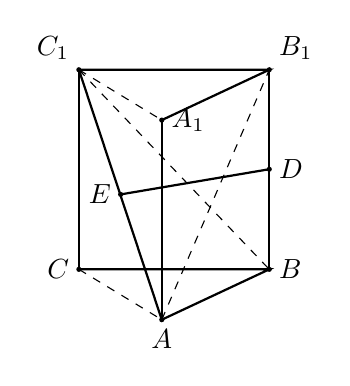
\begin{tikzpicture}[>=stealth,scale=0.78]
  \coordinate (A) at (2.20,0);
  \coordinate (B) at (3.95,0.82);
  \coordinate (C) at (0.85,0.82);
  \coordinate (A1) at (2.20,3.25);
  \coordinate (B1) at (3.95,4.07);
  \coordinate (C1) at (0.85,4.07);
  \coordinate (D) at (3.95,2.45);
  \coordinate (E) at (1.53,2.04);
  \draw[thick] (A)--(B)--(C);
  \draw[dashed] (C)--(A);
  \draw[thick] (A)--(A1) (B)--(B1) (C)--(C1);
  \draw[thick] (A1)--(B1)--(C1);
  \draw[dashed] (C1)--(A1);
  \draw[thick] (A)--(C1);
  \draw[dashed] (B)--(B1) (A)--(B1) (C1)--(B);
  \draw[thick] (D)--(E);
  \fill (A) circle (1.2pt) node[below] {$A$};
  \fill (B) circle (1.2pt) node[right] {$B$};
  \fill (C) circle (1.2pt) node[left] {$C$};
  \fill (A1) circle (1.2pt) node[right] {$A_1$};
  \fill (B1) circle (1.2pt) node[above right] {$B_1$};
  \fill (C1) circle (1.2pt) node[above left] {$C_1$};
  \fill (D) circle (1.2pt) node[right] {$D$};
  \fill (E) circle (1.2pt) node[left] {$E$};
\end{tikzpicture}
\end{center}
\nopagebreak[4]
（1） 证明：$ED$ 为异面直线 $BB_1$ 与 $AC_1$ 的公垂线；

（2） 设 $AA_1=AC=\sqrt2AB$，求二面角 $A_1-AD-C_1$ 的大小。

\Needspace{4\baselineskip}
\textbf{解析}

\Needspace{5\baselineskip}
设底面为 $z=0$，$B=(0,0,0)$，$A=(1,0,0)$，$C=(0,1,0)$，棱柱高为 $h$。则

\nopagebreak[4]
\[
B_1=(0,0,h),\quad A_1=(1,0,h),\quad C_1=(0,1,h),
\]

且 $D=(0,0,h/2)$、$E=(1/2,1/2,h/2)$。

\gksubpart{(1)}

\nopagebreak[4]
\[
\overrightarrow{DE}=\left(\frac12,\frac12,0\right)\perp BB_1\text{，}
\]

并且 $\overrightarrow{AC_1}=(-1,1,h)$，有 $\overrightarrow{DE}\cdot\overrightarrow{AC_1}=0$。直线 $DE$ 分别交 $BB_1,AC_1$ 于 $D,E$，所以是公垂线。

\gksubpart{(2)}

\Needspace{5\baselineskip}
条件 $AC=\sqrt2AB$ 与 $AB=BC$ 说明底面在 $B$ 处为直角，且可取 $AB=BC=1$、$h=\sqrt2$。平面 $A_1AD$、$ADC_1$ 的法向量可分别取

\nopagebreak[4]
\[
\boldsymbol n_1=(0,-\sqrt2,0),\qquad
\boldsymbol n_2=\left(-\frac{\sqrt2}{2},\frac{\sqrt2}{2},-1\right)\text{。}
\]

\Needspace{5\baselineskip}
于是两平面的锐角夹角满足

\nopagebreak[4]
\[
\cos\theta=\frac{|\boldsymbol n_1\cdot\boldsymbol n_2|}{|\boldsymbol n_1||\boldsymbol n_2|}=\frac12\text{，}
\]

故二面角为 $\dfrac\pi3$。

\gkanswer{答案（1）：见解析版}

\gkanswer{答案（2）：二面角 $A_1-AD-C_1$ 的大小为 $\dfrac\pi3$。}

\end{answer}
\begin{answer}
\gksolhead{20}{}

\textbf{题目}：

设函数 $f(x)=(x+1)\ln(x+1)$。若对所有的 $x\geqslant0$，都有 $f(x)\geqslant ax$ 成立，求实数 $a$ 的取值范围。

\Needspace{4\baselineskip}
\textbf{解析}

\Needspace{5\baselineskip}
对 $x>0$，

\nopagebreak[4]
\[
\frac{f(x)}x=\frac{x+1}{x}\ln(x+1)\text{。}
\]

由 $\ln(1+x)>\dfrac{x}{1+x}$（可由函数 $\ln(1+x)-\dfrac{x}{1+x}$ 的导数为 $\dfrac{x}{(1+x)^2}>0$ 得），有 $f(x)/x>1$。其下确界在 $x\to0^+$ 时为 $1$，因此对所有 $x\geqslant0$ 成立的充要条件为 $a\leqslant1$。

\gkanswer{答案：$a\leqslant1$。}

\end{answer}
\begin{answer}
\gksolhead{21}{}

\textbf{题目}：

已知抛物线 $x^2=4y$ 的焦点为 $F$，$A\text{、}B$ 是抛物线上的两动点，且 $\overrightarrow{AF}=\lambda\overrightarrow{FB}\ (\lambda>0)$。过 $A,B$ 两点分别作抛物线的切线，设其交点为 $M$。
\nopagebreak[4]
\begin{center}% 2006 年全国卷Ⅱ理科第 21 题：抛物线与两条切线
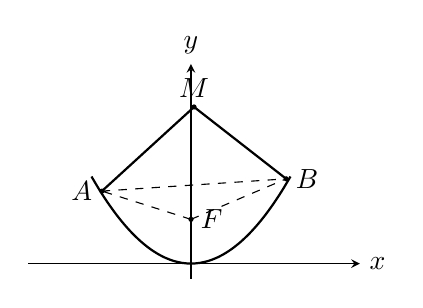
\begin{tikzpicture}[>=stealth,scale=0.78]
  \draw[->] (-2.65,0)--(2.75,0) node[right] {$x$};
  \draw[->] (0,-0.25)--(0,3.25) node[above] {$y$};
  \draw[thick] plot[smooth,domain=-2.25:2.25] ({0.72*\x},{0.28*\x*\x});
  \coordinate (F) at (0,0.72);
  \coordinate (A) at (-1.45,1.18);
  \coordinate (B) at (1.55,1.38);
  \coordinate (M) at (0.05,2.55);
  \draw[dashed] (A)--(B) (F)--(A) (F)--(B);
  \draw[thick] (A)--(M) (B)--(M);
  \fill (F) circle (1.2pt) node[right] {$F$};
  \fill (A) circle (1.2pt) node[left] {$A$};
  \fill (B) circle (1.2pt) node[right] {$B$};
  \fill (M) circle (1.2pt) node[above] {$M$};
\end{tikzpicture}
\end{center}
\nopagebreak[4]
（1） 证明 $\overrightarrow{FM}\cdot\overrightarrow{AB}$ 为定值；

（2） 设 $\triangle ABM$ 的面积为 $S$，写出 $S=f(\lambda)$ 的表达式，并求 $S$ 的最小值。

\Needspace{4\baselineskip}
\textbf{解析}

\gksubpart{(1)}

\Needspace{5\baselineskip}
令抛物线参数方程为 $P(t)=(2t,t^2)$，设 $A=P(t),B=P(u)$。焦点为 $F=(0,1)$，条件 $\overrightarrow{AF}=\lambda\overrightarrow{FB}$ 给出

\nopagebreak[4]
\[
t=-\lambda u\text{，}\qquad u^2=\frac1\lambda\text{，}\qquad tu=-1\text{。}
\]

\Needspace{5\baselineskip}
两条切线交点为 $M=(t+u,tu)=(t+u,-1)$。于是

\nopagebreak[4]
\[
\overrightarrow{FM}=(t+u,-2),\qquad
\overrightarrow{AB}=(u-t)(2,t+u)\text{，}
\]

从而 $\overrightarrow{FM}\cdot\overrightarrow{AB}=0$。

\gksubpart{(2)}

\Needspace{5\baselineskip}
又 $|u-t|=\sqrt\lambda+\dfrac1{\sqrt\lambda}$，且 $2+t^2+u^2=\left(\sqrt\lambda+\dfrac1{\sqrt\lambda}\right)^2$，故

\nopagebreak[4]
\[
S=\frac12\left(\sqrt\lambda+\frac1{\sqrt\lambda}\right)^3\geqslant4\text{。}
\]

最小值为 $4$。

\gkanswer{答案（1）：$\overrightarrow{FM}\cdot\overrightarrow{AB}=0$。}

\gkanswer{答案（2）：$S=f(\lambda)=\dfrac12\left(\sqrt\lambda+\dfrac1{\sqrt\lambda}\right)^3$，最小值为 $4$。}

\end{answer}
\begin{answer}
\gksolhead{22}{}

\textbf{题目}：

设数列 $\{a_n\}$ 的前 $n$ 项和为 $S_n$，且方程 $x^2-a_nx-a_n=0$ 有一根为 $S_n-1$，$n=1,2,3,\ldots$。

（1） 求 $a_1,a_2$；

（2） 求 $\{a_n\}$ 的通项公式。

\Needspace{4\baselineskip}
\textbf{解析}

\gksubpart{(1)}

\Needspace{5\baselineskip}
令 $S_0=0$。当 $n=1$ 时，根 $S_1-1=a_1-1$ 代入方程，或直接使用下式，得到 $a_1=\dfrac12$。一般地，把根 $S_n-1$ 代入

\nopagebreak[4]
\[
x^2-a_nx-a_n=0
\]

\Needspace{5\baselineskip}
并利用 $a_n=S_n-S_{n-1}$，可得

\nopagebreak[4]
\[
(S_n-1)^2-a_nS_n=0\text{，}\qquad
S_{n-1}=2-\frac1{S_n}\text{。}
\]

\Needspace{5\baselineskip}
因此

\nopagebreak[4]
\[
S_n=\frac1{2-S_{n-1}}\text{。}
\]

\Needspace{5\baselineskip}
由 $S_0=0$ 归纳得 $S_n=\dfrac n{n+1}$，于是

\nopagebreak[4]
\[
a_n=S_n-S_{n-1}=\frac1{n(n+1)}\text{。}
\]

\gksubpart{(2)}

特别地 $a_1=\dfrac12,a_2=\dfrac16$。

\gkanswer{答案（1）：$a_1=\dfrac12$，$a_2=\dfrac16$。}

\gkanswer{答案（2）：$a_n=\dfrac1{n(n+1)}$。}

\end{answer}